\paragraph{biguint-mul}

\subparagraph{Target}
Implement the multiplication of two biguints.

\subparagraph{Constraints logic}
\begin{itemize}
    \item Compute mul-factors first, use U32ArithmeticGate;
    \item Add mul-factors from low bits, use U32AddManyGate.
\end{itemize}

\subparagraph{Process layout}
See \figref{fig:biguint-mul-layout}
\begin{figure}[!ht]
    \centering
    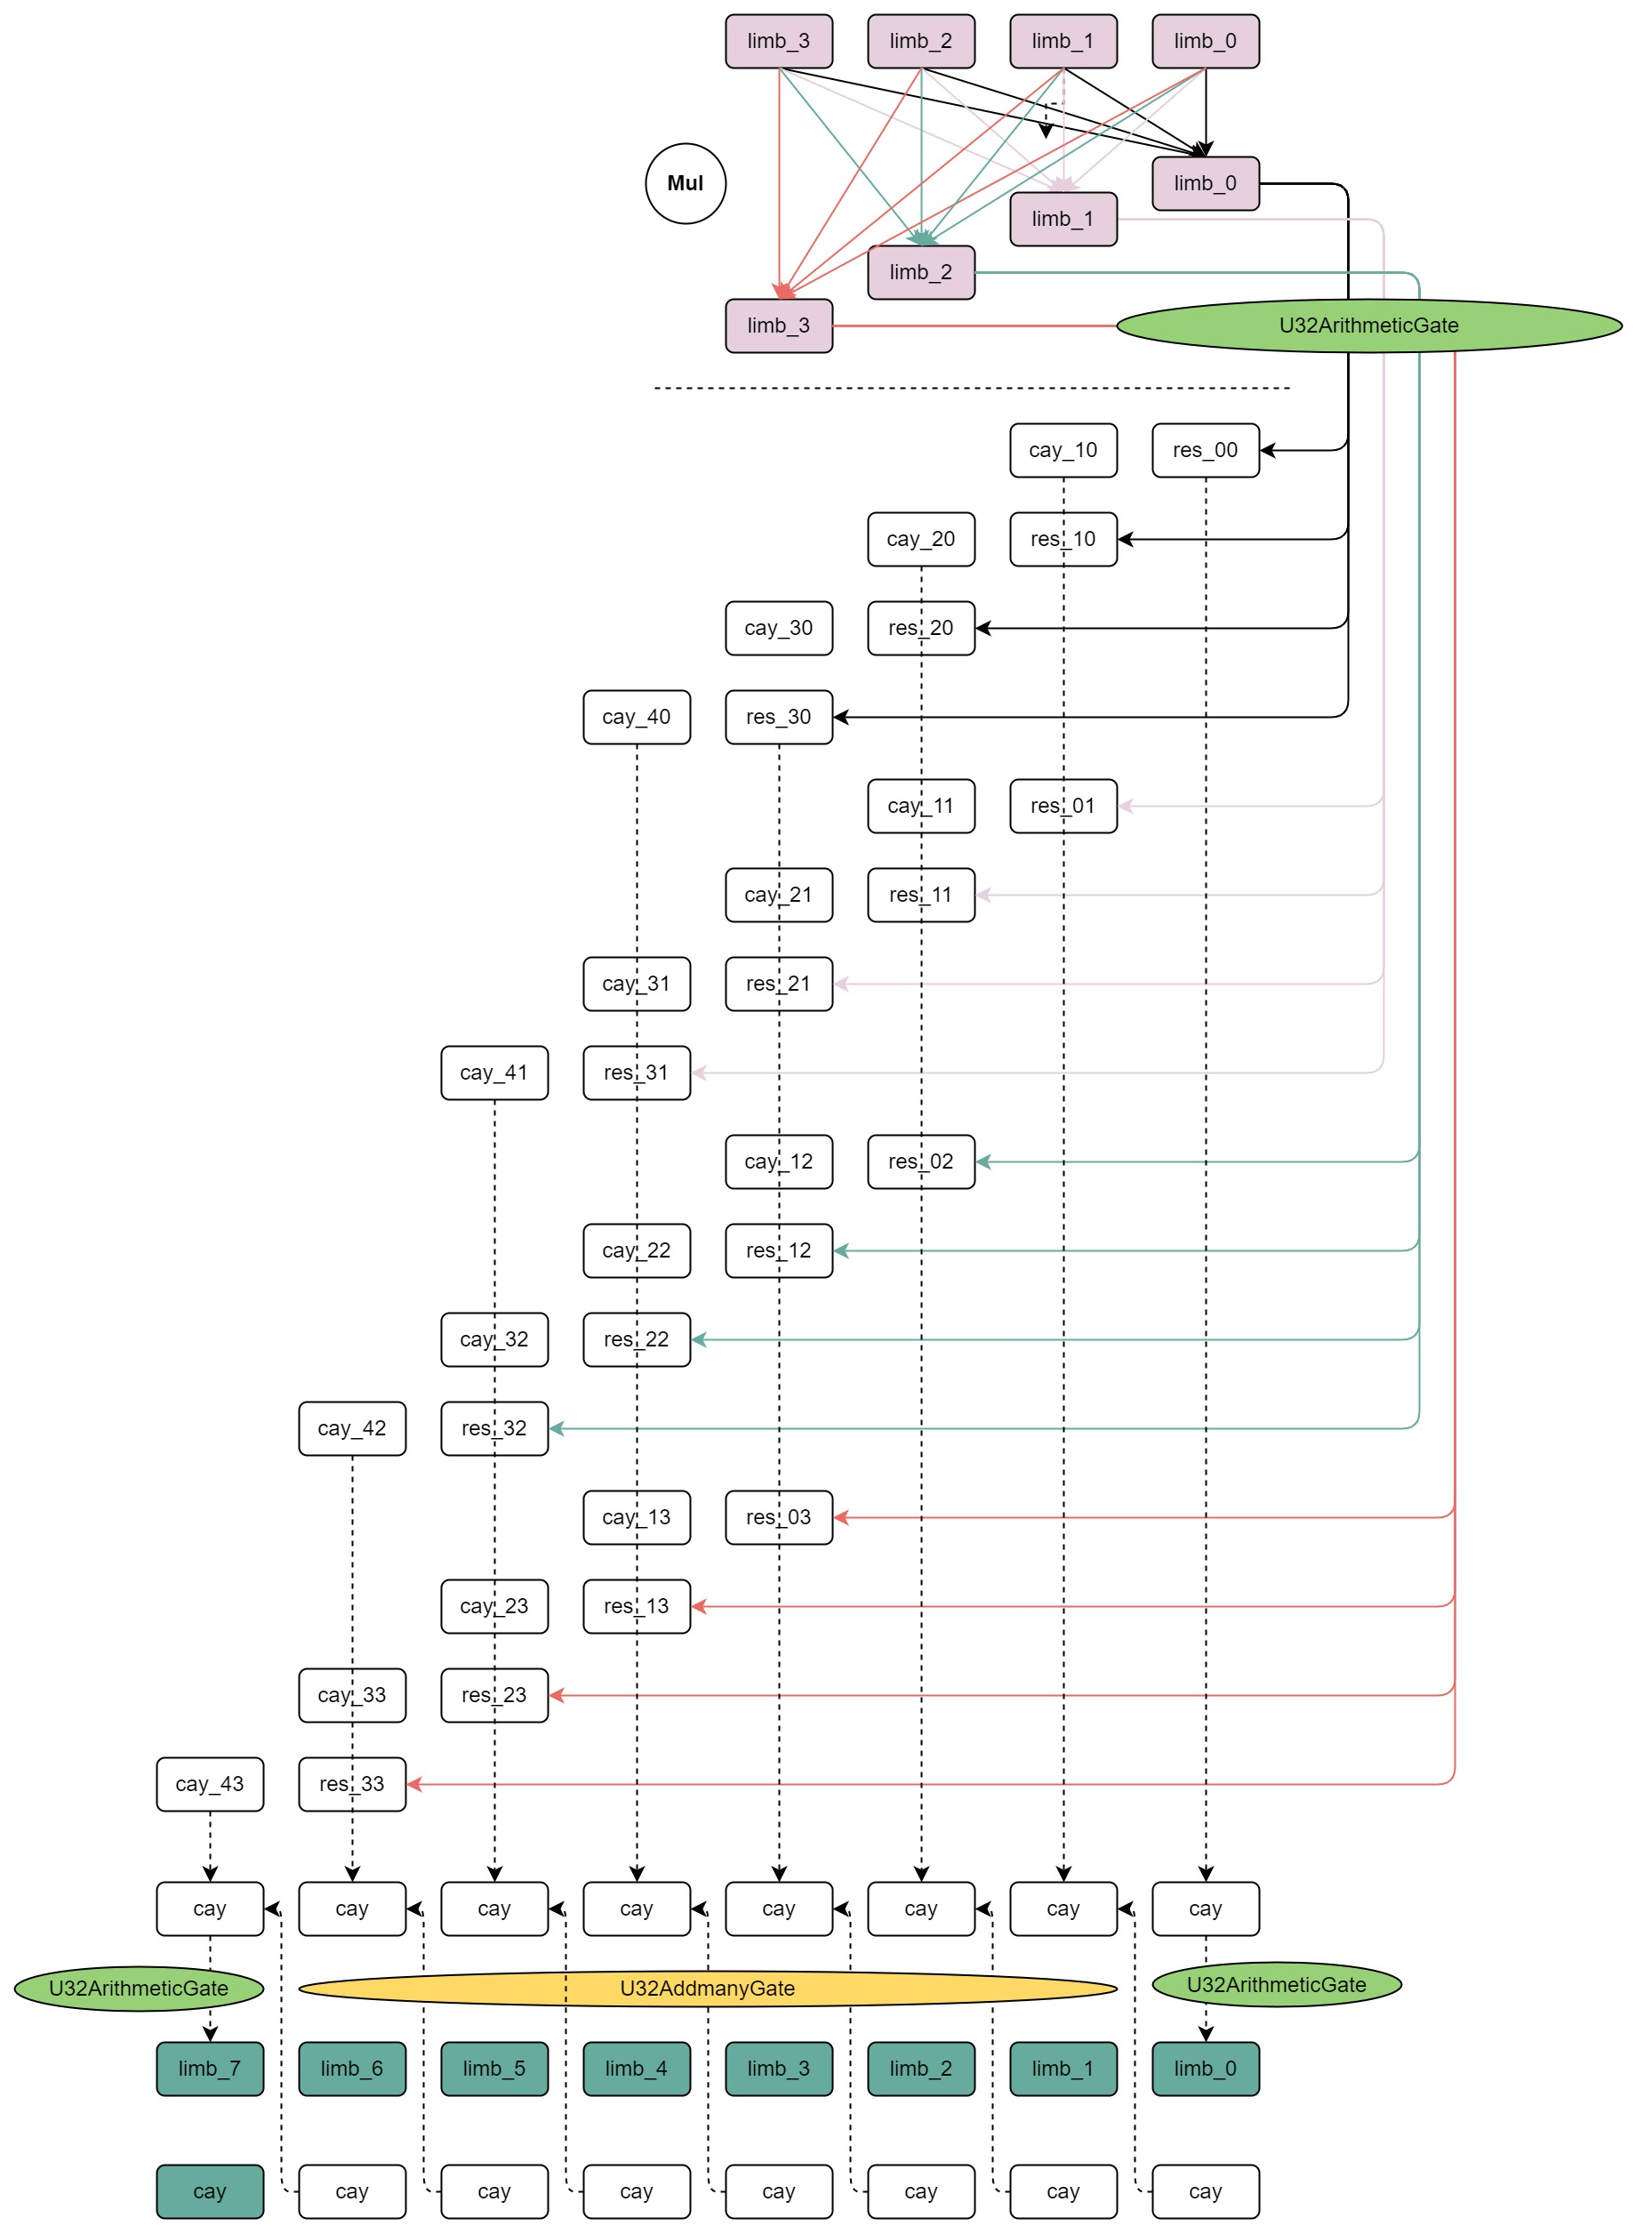
\includegraphics[width=0.6\textwidth]{biguint-mul-layout.jpg}
    \caption{biguint-mul layout}
    \label{fig:biguint-mul-layout}
\end{figure}

\subparagraph{Constraints info and costs}
\begin{itemize}
    \item Gate type num: 4 (U32ArithmeticGate, U32AddManyGate(num-addends: 4), U32AddManyGate(num-addends: 6), U32AddManyGate(num-addends: 8))
    \item Gate instance num: 9
    \item U32ArithmeticGate num: 6
    \item U32AddManyGate num: 3
    \item copy-constraints: $18 \times 3 + (4 + 6 + 8) \times 2 + 9 = 99$
    \item max-degree: 4
\end{itemize}
